\chapter{Problem Overview}


\label{sec:Intro}
\section{Introduction}

% Motivation
In the past few years there has been a lot of developments in the area of Big Data. Companies like Uber and Facebook handle large amounts of spatial data every day. This data can be used to improve service. For example, if we have taxi cab data, we might want to use this data to figure out the best locations for taxi cab stands. Good locations for taxi cab stands can result in less fuel consumption and lower wait times for the customers. A similar case can be made for medical emergencies and hospital locations. Even though, the cost of building a hospital is much higher than that of building a taxi station, the initial cost of building the infrastructure is assuaged over time if the location is beneficial. Companies like UPS are already saving millions of gallons of fuel per year by using Big Data Analytics. UPS uses On-Road Integrated Optimization and Navigation system(ORION) to determine the order of delivery, routes, and loading plans \citep{upsarticle}.

\begin{figure}[ht]
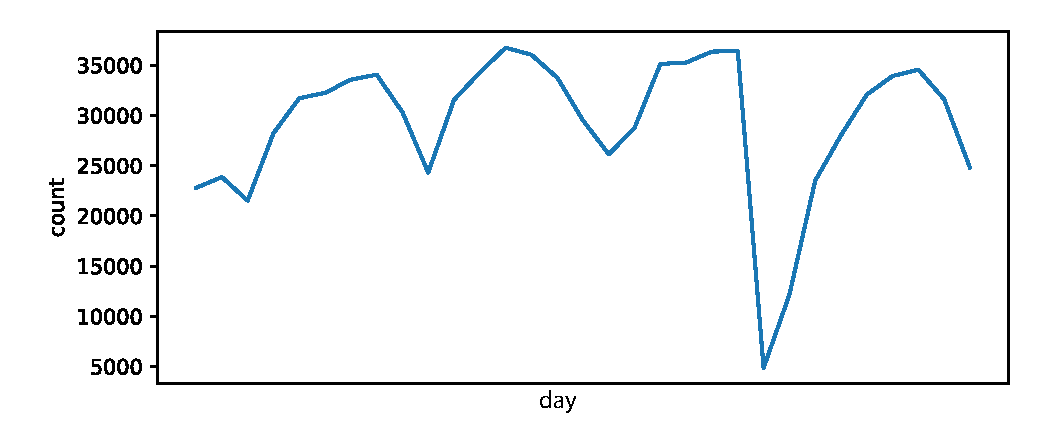
\includegraphics[width=\columnwidth]{yellowdata_count.eps}
\caption{Average number of yellow cab trips against the day for January 2016}
\label{fig:yellowstats}
\end{figure}

The New York City Taxi and Limousine Commission (NYC TLC) regulates yellow cab taxis\citep{taxi2016tlc}. It has licensed around 146,000 distinct drivers. In order to view a demonstration of the database explanation system, we can use this dataset. The Yellow Cab data has several attributes including spatial attributes such as latitude, longitude and non spatial attributes such as tip amount and total amount for each trip. Fig.~\ref{fig:yellowstats} shows the number of yellow cab trips against time for January 2016. The sharp decline in the number of trips in the last quarter of the month is pronounced. One might be inclined to look up the date when the number of trips crashed. In this paper, we look at different approaches to explain these types of observations. In fact, we also look at observations with a spatial dimension.

Whenever we analyze some data, we might be tempted to find out a reason for specific observations. While some data observations might be interesting, in order to make decisions based on these observations, one might find it useful to find an explanation. For example, someone looking to start a business might look at locations in which their specific category of business succeeds. It might be even more beneficial to find out why it prospers in that specific location.

This thesis describes a system that we have created to explain database observations. Our system intends to produce spatial explanations. There are two types of input to our system. One of the inputs is the dataset we want to analyze. The second input is our observation. The observation can be in the form of an aggregate query. Our system uses one of several different solutions to find an explanation depending on what the user wants. The output of our system is an explanation for our system based on predicates.

The explanations produced by our system are formally defined later on in this document. However, it is important to introduce the basic idea so the reader can follow along. In our proposed system, explanations are parts of the data that have a significant effect on what we are observing. For example, if we are observing tips for taxi trips and removing a few tuples from the dataset has a significant effect on the tips, then the few tuples would be considered as an explanation for our observation. Another definition of explanations in our proposed solution involves looking at different parts of the data. For example, if we divide our data into a number of parts, the parts which deviate from the average value of tip percentage are considered as explanations because they introduce the largest differences.

In this thesis we define a taxonomy(Section~\ref{sec:taxonomy}) for observations and explanations.  The observation we made in Fig.\ref{fig:yellowstats} can be considered as a non spatial observation. Its explanation can either be non spatial or spatial. The first class in our taxonomy deals with non spatial explanations for non spatial observations(Section~\ref{sec:nonspatial_nonspatial}). The second class is related to spatial explanations for non spatial observations(Section~\ref{sec:spatial_nonspatial}) while the last class is about spatial explanations for spatial observations. Many geospatial datasets that we encounter contain time as one of the attributes. When we talk about spatial explanations, we do not take time into consideration. Instead, time is considered as a non-spatial attribute.

There are three main approaches to explanation that we study in this thesis. Each approach has been extended to satisfy our taxonomy. Each approach relies on the fact that the observation is an aggregated attribute in our data set while the explanation is a predicate. \textbf{Aggravation}(Section~\ref{sec:aggravation}) is based on the principle that if we consider only the tuples in our database satisfying our explanation predicate, the value of the observation on our modified dataset will be our measure of aggravation\citep{roy2014formal,meliou2014causality}.

In contrast, \textbf{Intervention}(Section~\ref{sec:intervention}) measures the influence of our explanation i.e. what will be the value of our observation when all the tuples satisfying our explanation predicate are removed\citep{roy2014formal}. We also extend Intervention to introduce \textbf{Hierarchical Intervention}(Section~\ref{sec:hei_intervention}). This approach measures the value of intervention when the explanation consists of a cluster of spatial polygons in our explanation predicate.

Finally, \textbf{Salient Features}(Section~\ref{sec:salient_features}) can be used to find explanations\citep{chirigati2016data}. Each salient feature encapsulates a polygon where an attribute in the dataset is pronounced. The correlation between a salient feature of the observation and the salient feature of the explanation can give us possible explanations.

Each approach has its own set of advantages and disadvantages. While one approach might give us very specific explanations that show a textbook example of our observation, another might give us an explanation which is hard to see in the context of the observation but has a large overall impact on it. One of the objectives of this paper is to compare which approach is suitable considering its context.

We implemented(Section~\ref{sec:implementation}) these approaches, including hierarchical intervention using distributed data frameworks\citep{borthakur2007hadoop,dean2008mapreduce,shanahan2015large,zaharia2016apache}. We made optimizations in our implementation to make sure our approach is orders of magnitude faster than the naive approach. The implementation of salient features was used from the Data Polygamy framework \citep{chirigati2016data}.

In order to compare each approach, we defined a few evaluation metrics. The \textbf{Intensity}(Section~\ref{sec:intensity}) metric measures how relevant each explanation is to the observation. To be more specific, it measures the value of the observation for the top explanations for each approach. The \textbf{Influence}(Section~\ref{sec:influence}) metric measures the observation when the top explanation is removed from the data. We also compare the speed(Section~\ref{sec:speed}) of our implementations of each approach.

\section{Related Work}
There has previously been some work related to database explanations. Most of this work revolves around the notion of causality. There is existing work in the field of Artificial Intelligence by \cite{zhang2002discovering} which expresses relationships between different attributes in a dataset as conditional probabilities. Based on the conditional probability each tuple is given a set of binary rankings.

The work by \cite{meliou2010causality} is a survey which looks at causality from the perspective of a database problem. Traditionally, work on causality from the database perspective mainly deals with provenance i.e. events which occurred chronologically. This solution, however, only works with databases with timestamps. This paper also looks at the degree of responsibility which is defined as the number of tuples which have to be removed to change a binary observation. An example of a binary observation is winning and losing an election for instance. If a candidate wins by a high margin, each tuple has a lower degree of responsibility. On the other hand a close victory for a candidate increases each voters degree of responsibility.

The paper by \cite{meliou2014causality} is a survey of work in causality and explanations in both the Artificial Intelligence and Database communities. The take away from this survey is that AI problems tend to have a bigger causal network while database problems tend to have more variables.

There has also been a lot of work on correlation which shares some common ground with the work on explanations. One interesting recent work on the subject is the Data Polygamy framework\citep{chirigati2016data}. This framework is designed to find the correlation between a corpus of datasets. It uses the peaks and troughs of the data to calculate \textit{salient features} \citep{dunn1986applied}. The positive and negative correlation between these salient features can be used to decide whether dataset are related\citep{su2014supporting}. The objective of our system is a bit different from finding corelations. There are a number of different factors which can effect observations. Correlation might be one of these attributes in certain cases but if we ignore other criteria such as selectivity then we might get results which do not have a significant impact. E.g. if two attributes are highly corelated in a certain spatial cluster but the selectivity of the cluster is small, it would lead to a low impact on the observation.

There has also been work related to why not explanations in databases. The work by \citep{ten2015high} looks at the question of why some tuples are missing from database results. This paper uses the assumption that the relationship between tuples is defined in the form of an ontology. The paper uses the relationship between the ontology for a schema and the ontology for an instance of the schema to judge whether an explanation exists. The ontologies that are used can be created manually or automatically. Using provenance \citep{cheney2009provenance} can help in creating ontologies.

Our solution mainly builds upon work by \cite{roy2014formal} which outlines a formal approach to explain data. The main solutions outlined in that work are Aggravation and Intervention. The work by \cite{roy2014formal} is designed to work with non spatial datasets. One of the main points of the paper is that their approach works on a dataset which can span several tables related by primary and foreign keys. While the approach outlined by \cite{roy2014formal} is great for non spatial data, it does not translate well in the spatial domain. This approach develops on previous work in causality and influence. It also resembles data mining concepts related to association rule mining\citep{agarwal1994fast,tan2006introduction}. In association rule mining sets of attributes that occur together are assigned a support and confidence. The support measures the frequency of occurrence of a set of attributes while confidence measures how frequently an attribute occurs with another set of attributes. The work by \cite{koperski1995discovery} looks at association rule mining in a spatial context. Given a set of spatial relationships, it applies association rule mining to find relationships that frequently occur together. There is a difference between association rule mining and our prosposed approach. First of all, our proposed approach uses a user defined observation. Secondly, in our approach we are not looking at the associations but rather at the effect of removing or filtering pieces of data. A high association between predicates does not necessarily mean that removing them will significantly effect the observation.

Spatial Analysis is very popular in GeoScience and GeoInformatics. Regression techniques can be used to explain data\citep{dunn1986applied,cleveland1988locally}. The idea behind regression techniques is to express an attribute that we are interested in as a dependent variable. This dependent variable can then be expressed in the form of parametric equation involving other attributes in the dataset as independent variables. An example of a loss function for this kind of regression is Ordinary Least Squares(OLS)\citep{dismuke2006ordinary}. The user of this system decides a dependent variable and a set of explanation variables. The resulting equation has coefficients assigned to each explanatory variable as well as a bias term. This results in a curve fitting problem. The curve fitting problem is solved using regression i.e. the coefficient terms and the bias are iteratively adjusted until the sum of squared error between the predicted curve and the ground truth results in a minimum value. Regression techniques are widely used for spatial data analysis. However, they depend on predefined spatial partitioning and look at the data as a whole rather than looking at it from the perspective of a user defined observation compared to our solution.

Geographically Weighted Regression(GWR) expands on OLS regression for geospatial data\citep{brunsdon1998geographically,charlton2009geographically}. GWR tries to use the regression equation for each feature in the dataset. It uses the idea that spatially co-located points contribute more to each other by using a spatially aware kernel function. A kernel function like a Gaussian, for example, gives more weight to nearby points than to points which are far apart.

Besides work related to explanation, there has been a lot of research in the area of spatial correlation. Much of the work in this area extends from multiple old works by Getis\citep{getis1991spatial,ord1995local,getis1996local,getis2002comparative,getis2007reflections}. The Getis Ord statistic \citep{ord1995local} for example is useful in showing us areas with high local spatial associations. The Moran's I statistic is useful for measuring the spatial heterogeneity of the data\citep{assuncao1999new,zhang2008use}. Moran's I is useful in hot spot analysis which can be viewed as a step in the way of finding explanations.

\section{Contributions}

In this paper we extend several approaches and compare them. There are three major contributions in this thesis:
\begin{itemize}

\item We extend aggravation and intervention for spatial explanations/observations. Aggravation and Intervention techniques in literature are designed for giving non spatial explanations for non spatial observation. When we look at spatially heterogeneous data, the spatial context has impact on the value of the explanations.

\item We extend the use of salient features to give spatial explanations for simple observations based on attributes. Salient Features can be used to compare the correlation between attributes between multiple datasets. However, we re purpose the use of salient features for explanations. We use the salient features for attributes in the same dataset to form explanations.
\item We introduce a new approach: Hierarchical Intervention. This approach uses spatial partitioning/clustering. We find that there is a difference between explanations for spatially heterogeneous data for different dimensions of spatial explanations. Therefore, we propose a new approach which uses a spatial hierarchy. This accounts for explanations for multiple dimensions of the data.

\item We introduce a method to balance influence and intensity to give better explanations. Influence and Intensity measure the global and local impact of an explanation, respectively. We acknowledge that the user of our system can have a non binary preference for either. We construct our system in a way that it produces explanations as a linear relationship between influence and intensity.

\item We introduce an automated system for giving explanations based on our findings. The system that we have defined has a lot of parameters. It requires observations, coefficients, arithmetic relationships and selectivities as parameters. We have designed a Web based User Interface to help a user with little knowledge of the system to get explanations for their observations.
\end{itemize}

% The approaches that we mention in his paper borrow from previous work on explanation and correlation. We have extended existing frameworks to work on our specific taxonomy. Aggravation(Section~\ref{sec:aggravation}) and Intervention(Section~\ref{sec:intervention}), for instance, are approaches which are originally designed to work in a non spatial context. They provide explanations in the form predicates over attributes. If we have a dataset with latitude and longitude as the spatial attributes, they may provide explanation in terms of just a latitude or longitude as separate continuous attributes. They might even provide explanations with no spatial attributes at all. Another drawback of using these approaches with spatial data is that they function without any knowledge of spatial locality.
%
% We highlight a new approach called hierarchical intervention (Section~\ref{sec:hei_intervention}). This approach intends to use clusters of spatially co located points or polygons in an attempt to come up with better explanations. As the name suggests, this approach borrows from the intervention approach. It uses spatial partitioning to improve spatial explanations.
%
% Another contribution of this paper is outlining a method for using salient features for explanations. The salient features approach is originally intended to work for correlation between datasets. Our extension of this approach intends to use it for the purpose of explanations. Extending salient features for explanation rather than correlation involves some additional step of work while discarding parts of the previous work which relates specifically to correlation. The original work uses salient features to compare multiple datasets and rank the most correlated datasets. Our usage of salient features is intended to explain only a single dataset with multiple attributes. Even if two attributes of a dataset are highly correlated, it may or may not rank the two attributes in the top explanations depending on the observation.

One of the contributions of this thesis is to compare the different approaches. In order for us to compare different things, we need to do so on the basis of a common standard. The different solutions to the explanation problem are structurally very different from each other. As previously mentioned, some of them are originally not designed to handle spatial data. We have designed a common taxonomy to compare all these different solutions. On top of designing this taxonomy, our extension of each approach is designed to make sure each solution adheres to the taxonomy. Even though, this still leaves room for differences between each solution, it gives us room for comparison.

We also define a number of evaluation metrics and an approach which uses them to come up with better explanations.

% \section{Document Outline}
%
% This section is intended to  give an outline of the remaining document:
%
%
% Chapter~\ref{chp:prelims} goes over the various nomenclature, tools, and techniques that we use throughout the paper.
%
% Chapter~\ref{chp:architecture} goes over the taxonomy for our observation/explanation system. It goes over the different kinds of observations and explanations. It also goes over different explanation techniques in literature, how they compare, and their significance for different contexts.
%
% Chapter~\ref{chp:proposed} deals with outlining our proposed system. It goes over an outline of our proposed system. Gives an explanation of various clustering schemes that we use. We also go into the implementation details of our system in this chapter. Finally, we go over the user interface that we have designed to interact with our system.
%
% Chapter~\ref{chp:eval} gives details about the various experiments we performed as well as the evaluation for our proposed system.
%
% Chapter~\ref{chp:concl} gives concluding remarks about this work as well as ideas about future work.
